\documentclass[crop,tikz]{standalone}% 'crop' is the default for v1.0, before it was 'preview'
%\usetikzlibrary{...}% tikz package already loaded by 'tikz' option
\begin{document}
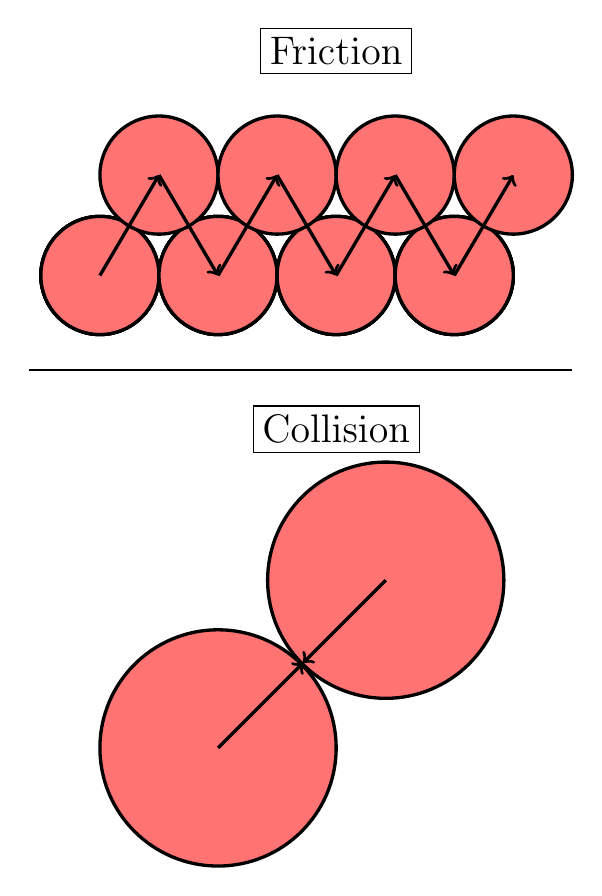
\begin{tikzpicture}[scale = 1.5]
    % \draw (-11.5,4) node {\textbf{A}};
    % \draw (-1.5,4) node {\textbf{B}};

    \def \b {-7};
    \def \c {0.1};
    \def \d {0.1};
    \def \r {2.3};

    \draw[color=black, fill=red!55, very thick] (-5, -3.7) circle (1);
    \draw[color=black, fill=red!55, very thick] (-5 + 1.42, 1.42-3.7) circle (1);
    \draw[->, very thick] (0-5, 0-3.7) -- (0.72-5, 0.72-3.7) ;
    \draw[->, very thick] (1.42-5, 1.42-3.7) -- (0.72-5, 0.72-3.7 );

    \node[draw] at (-4,2.2) { \Large Friction};
    \node[draw] at (-4,2.7-3.7) { \Large Collision};

    \foreach \x in {1, ..., 4}
        \foreach \y in {1.5, ..., 4.5}
            \draw [color=black, fill=red!55,very thick] (\x + \b, 0.3) circle (0.5);

            
    \foreach \x in {1.5, ..., 4.5}
            \draw [color=black, fill=red!55, very thick] (\x + \b, 1.15) circle (0.5);

    \foreach \x in {1, ..., 4}
            \draw [very thick, ->] (\x + \b, 0.3) -- (\x + \b + 0.5 , 1.15);

    \foreach \x in {1.5, ..., 3.5}
        % \foreach \y in {1, ..., 4}  
            \draw [->, very thick] (\x + \b, 1.15) -- (\x + \b + 0.5 , 0.3); 


    \draw [line width = 1pt] (-6.6,-0.5) -- (-2,-0.5); 

    
    % \foreach \x in {3, 4, ..., 5}
    %     \foreach \y in {0, 1, ..., 3}        
    %         \draw (\x - \d, \y - \c) circle (0.5);
\end{tikzpicture}
\end{document}